\let\negmedspace\undefined
\let\negthickspace\undefined
\documentclass[journal]{IEEEtran}
\usepackage[a5paper, margin=10mm, onecolumn]{geometry}
\usepackage{lmodern} % Ensure lmodern is loaded for pdflatex
\usepackage{tfrupee} % Include tfrupee package

\setlength{\headheight}{1cm} % Set the height of the header box
\setlength{\headsep}{0mm}     % Set the distance between the header box and the top of the text

\usepackage{gvv-book}
\usepackage{gvv}
\usepackage{cite}
\usepackage{amsmath,amssymb,amsfonts,amsthm}
\usepackage{algorithmic}
\usepackage{graphicx}
\usepackage{textcomp}
\usepackage{xcolor}
\usepackage{txfonts}
\usepackage{listings}
\usepackage{enumitem}
\usepackage{mathtools}
\usepackage{gensymb}
\usepackage{comment}
\usepackage[breaklinks=true]{hyperref}
\usepackage{tkz-euclide} 
\usepackage{listings}
\def\inputGnumericTable{}                                 
\usepackage[latin1]{inputenc}                                
\usepackage{color}                                            
\usepackage{array}                                            
\usepackage{longtable}                                       
\usepackage{calc}                                             
\usepackage{multirow}                                         
\usepackage{hhline}                                           
\usepackage{ifthen}                                           
\usepackage{lscape}

\begin{document}

\bibliographystyle{IEEEtran}
\vspace{3cm}

\title{10.4.4.2.2}
\author{EE24BTECH11036 - Krishna Patil}
% \maketitle
% \newpage
% \bigskip
{\let\newpage\relax\maketitle}

\renewcommand{\thefigure}{\theenumi}
\renewcommand{\thetable}{\theenumi}
\setlength{\intextsep}{10pt} % Space between text and floats

\renewcommand{\thefigure}{\theenumi}
\renewcommand{\thetable}{\theenumi}
\setlength{\intextsep}{10pt} % Space between text and floats

\textbf{Question}: Find the values of k for following quadratic equations, so that they have two equal roots : 
\begin{align}
	kx(x-2) + 6 = 0
\end{align}

\solution
For equal roots of a quadratic equation, the discriminant is zero i.e., For the quadratic $ax^2 + bx + c =0$ the discriminant $b^2 - 4ac = 0$ .
\begin{align}
	kx(x-2) + 6 &= 0 \\
	kx^2 -2kx + 6 &= 0 \\
	\therefore a = k, b = -2k, c &= 6 \\ 
	\therefore 4k^2 -24k &= 0 \\
	k = 0 \quad or \quad k = 6
\end{align}
but $k = 0$ doesn't make sense as no solution is obtained so, $k = 6$ is the answer. 

So, the equation becomes
\begin{align}
	6x(x-2) + 6 &= 0 \\
	6x^2 - 12x + 6 &= 0 \\
	x^2 - 2x + 1 &= 0
\end{align}

\begin{enumerate}
	\item \textbf{Thereotical Solution} : \\
		\begin{align}
			x^2 - 2x + 1 &= 0 \\ 
			(x-1)^2 &= 0 \implies x = 1 
		\end{align}
	\item \textbf{Numerical Solution} : \\
	
		\begin{enumerate}
			\item \textbf{Fixed point iteration Method} : \\
				Say , we have to find roots of 
					\begin{align}
						f\brak{x}=0
					\end{align}
				using algebra, we first solve  for $x$ i.e., $x = g\brak{x}$ where, $g\brak{x}$ is some other function formed after solving.
				then we select an initial guess \( x_0 \), iterate using the formula 
					\begin{align}
						x_{n+1} = g(x_n)
					\end{align}
				Repeat this step until the difference between successive approximations $ \abs{x_{n+1} - x_n} $ is less than a specified tolerance  $\epsilon$.

				\newpage

				say for our case , we choose $\epsilon = 10^{-6}$ and $x_0 = 1.5$ and $f\brak{x} = x^2 -2x + 1 $,
					\begin{align}
						\because f\brak{x} &= 0 \\
						x^2 - 2x + 1 &= 0 \\
						\sqrt{2x - 1} &= x \\
						\therefore g\brak{x} &=  \sqrt{2x - 1} 
					\end{align}
				So, the iterative equation is ,
				\begin{align}
					x_{n+1} = \brak{\sqrt{2x_n - 1} }	
				\end{align}
				after computing , we obtain $x = 1.0014142$ which is pretty near to the theoretical solution. \\

			\item \textbf{Newton-Raphson Method}
				
				The Newton-Raphson method is an iterative technique to find the roots of a real-valued function \( f(x) \). The update formula is given by:

					\begin{align}
						x_{n+1} &= x_n - \frac{f(x_n)}{f'(x_n)}
					\end{align}

				For the function \( f(x) = x^2 - 2x + 1 \), the derivative is:

					\begin{align}
						f'(x) &= 2x - 2
					\end{align}
					\begin{align}
						f(x) &= x^2 - 2x + 1 \\
						f'(x) &= 2x - 2
					\end{align}
				The Newton-Raphson update formula becomes:
					\begin{align}
						x_{n+1} &= x_n - \frac{x_n^2 - 2x_n + 1}{2x_n - 2}
					\end{align}
				After computing , we obtain $x = 0.999999$ which is pretty near to the solution. \\ 
		\end{enumerate}
		
	

\begin{figure}[htbp]
           \centering
        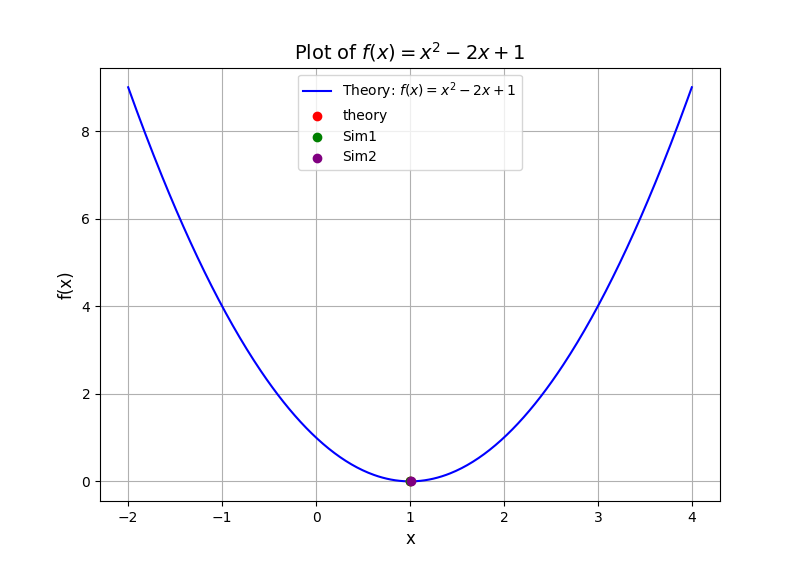
\includegraphics[width=\textwidth]{fig/Figure_1.png} % Replace with your figure file
                \label{fig:fig1}
    
    \hspace{0.05\textwidth}
    
          \centering
        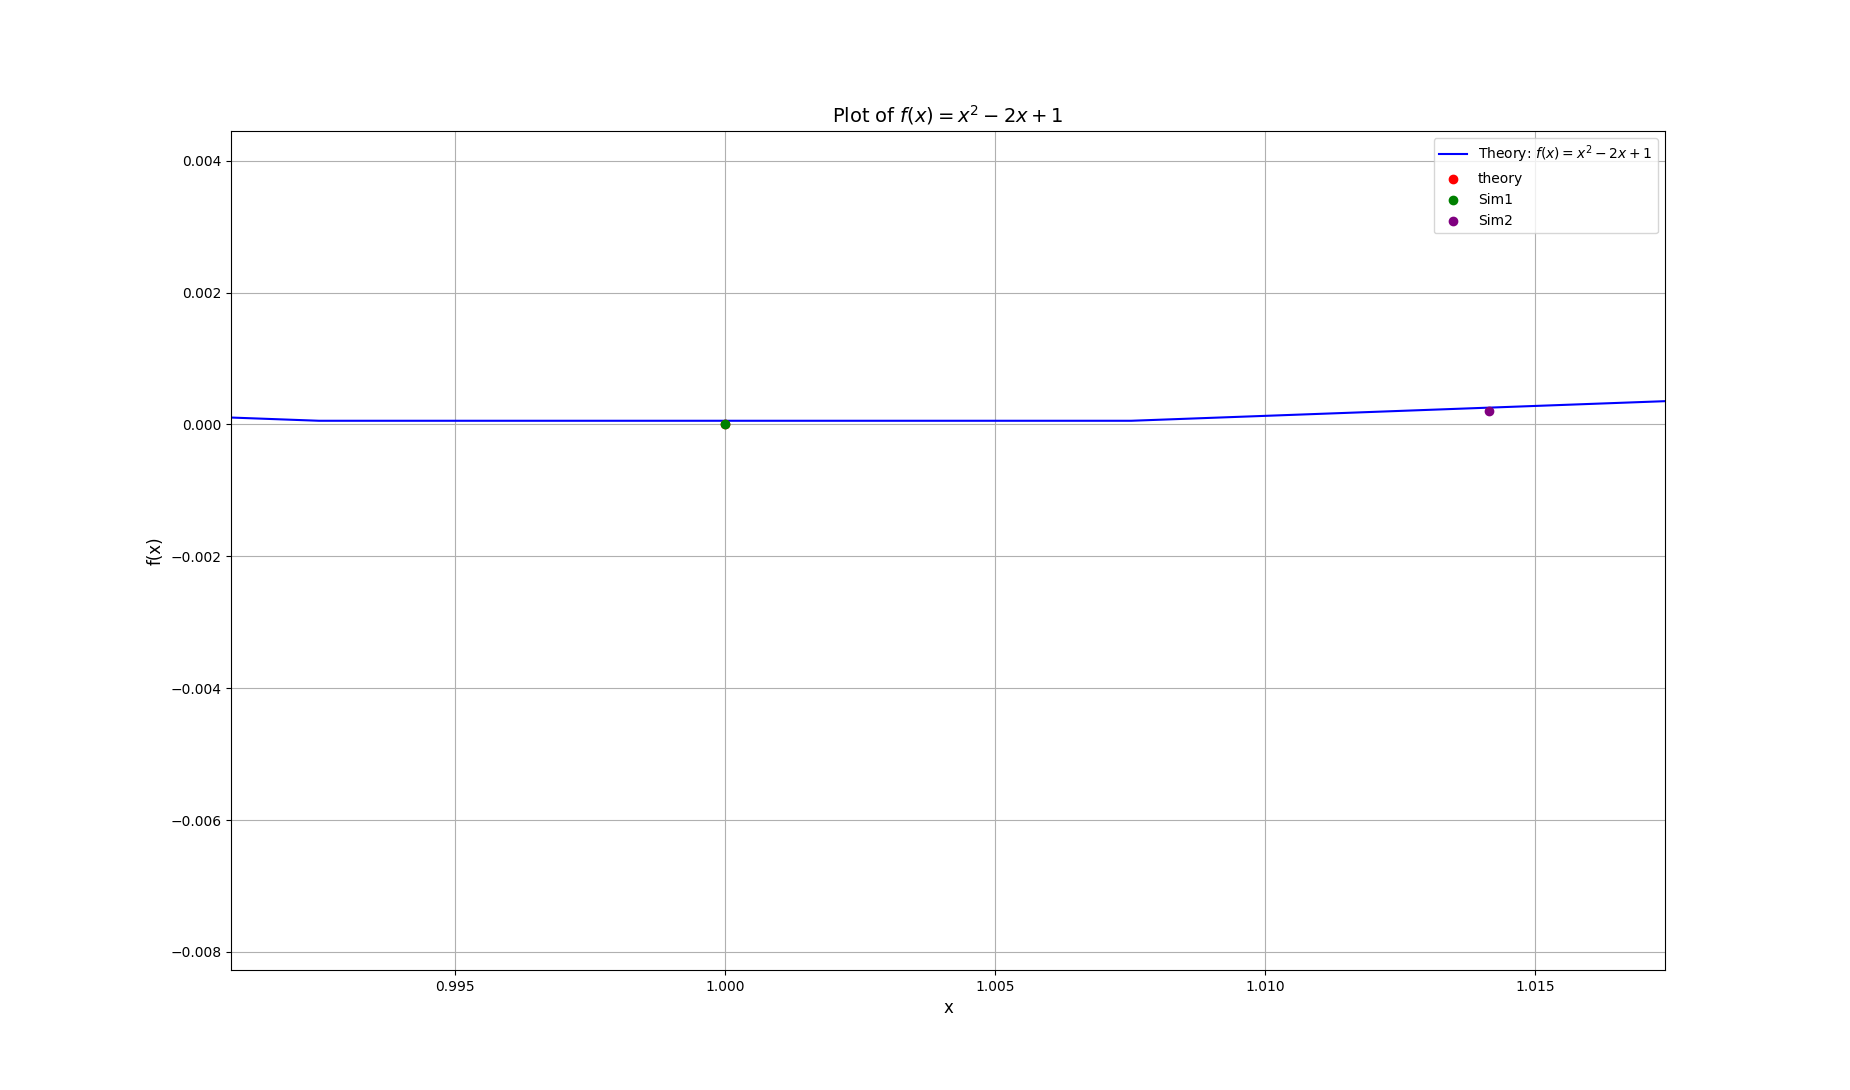
\includegraphics[width=\textwidth]{fig/Figure_2.png} % Replace with your figure file
        \caption{Zoomed Form}
        \label{fig:fig2}
   \end{figure}


\end{enumerate}
\end{document}
